\documentclass[xcolor={usenames,dvipsnames}]{beamer}

\usepackage[utf8x]{inputenc}

\definecolor{solarbg}{HTML}{FDF6E3}

\usepackage{minted}
\newminted{c}{frame=single}
\usemintedstyle{solarized}

\usetheme{Antibes}
\usecolortheme[named=Bittersweet]{structure}

\title[Glift: Generic, Efficient, Random-Access GPU Data Structures]%
      {Glift:\\ Generic, Efficient, Random-Access GPU Data Structures}
\author{Aaron E. Lefohn et al. -- University of California, Davis}
\institute{By Jean Niklas L'orange,
  \\for the course TDT24 at the Norwegian University of Science and Technology}
\date{October 15, 2013}

\begin{document}

\begin{frame}
  \titlepage
\end{frame}

\section{What and why?}
\begin{frame}
  \frametitle{What is this paper about? What is Glift?}

  This paper is about a data-parallel programming abstraction. The abstraction
  enables GPU programmers to write high-level, efficient random-access GPU data
  structures, without sacrificing performance.

  \vfill \pause

  Glift is an implementation of that abstraction, using C++/Cg/OpenGL.
\end{frame}

\begin{frame}
  \frametitle{Paper Structure}

  This paper is structured into several parts:
  \begin{itemize}
  \item<2-> Rationale, considerations and the abstraction itself
  \only<6->{\item<5-> \textcolor{gray}{(Glift programming)}}
  \item<3-> Classification of existing GPU data structures based on the
    abstraction
  \item<4-> Case studies
  \item<5-> Results, discussion, conclusions
    \mode<beamer|second|trans|article>{\only<-5>{\item<6->}}
  \end{itemize}
\end{frame}

\section{Rationale, considerations, the abstraction}
\subsection{Rationale}
\begin{frame}
  \frametitle{Rationale}

  Why is a data structure abstraction desirable? Two main reasons:
  \begin{enumerate}
  \item<2-> Code reuse -- No need to copypaste existing data structures
  \item<3-> Decouple data structures and algorithms → reduce complexity
  \end{enumerate}
\end{frame}

\subsection{Considerations}
\begin{frame}
  \frametitle{Considerations}

  Several things which have been taken into consideration when abstraction was
  designed:
  \begin{itemize}
  \item<2-> Incremental adoption
  \item<3-> Extensibility
  \item<4-> Efficiency
  \item<5-> CPU/GPU interoperability
  \end{itemize}
\end{frame}

\subsection{The Abstraction}
\begin{frame}
  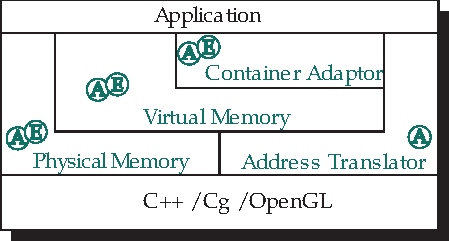
\includegraphics[width=\linewidth]{img/glift-components}
\end{frame}

\begin{frame}
  \frametitle{Virtual memory → Address translator → Physical memory}
  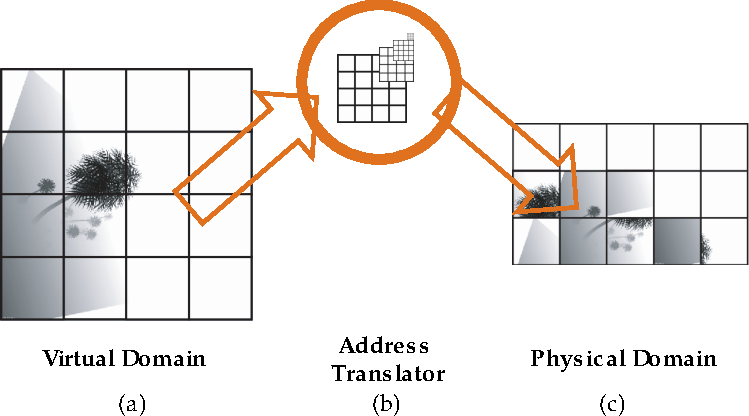
\includegraphics[width=\linewidth]{img/addr-translator}
\end{frame}

\begin{frame}
  \frametitle{Iterators}

  The last component of Glift is iterators. Based on C++'s iterator, they
  designed GPU iterators for parallel work. There are two types of iterators:
  \begin{itemize}
  \item<2-> Element Iterators -- for iterating over the elements in the
    structure
  \item<3-> Address Iterators -- enables address translators to specify
    iteration without having knowledge of physical data
  \end{itemize}
\end{frame}

\begin{frame}[fragile]
  \frametitle{Iterators -- example}
  \inputminted[frame=single]{c}{code/laplace.c}
\end{frame}

\section{Classification of GPU data structures}
\begin{frame}
  \frametitle{Classification of GPU data structures}

  The authors classify different data structures in terms of Glift concepts.
  \begin{itemize}
  \item<2-> ND-to-MD translators -- done analytically
  \item<3-> Page Table translators -- using the page tables on the GPU
  \item<4-> GPU tree structures -- $k$-d trees, quadtrees, octrees\ldots
  \item<5-> Dynamic GPU structures -- usually adaptive and sparse
  \end{itemize}
  \onslide<6->{Usually easy to create different structures with Glift, but some
    are challenging to port.}
\end{frame}

\section{Case Studies}
\begin{frame}[fragile]
  \frametitle{Case Studies}

  \only<1,3->{\vspace{15mm}
    We've already seen one! \vspace{3mm}

    \uncover<3->{Also describes a GPU stack. While simple, is useful for e.g.
      $k$-d tree traversal.\vspace{3mm}}

    \uncover<4->{Covers the implementation details of dynamic multiresolution
      adaptive data structures for real time usage, and implements both adaptive
      shadow maps and octree 3D paint as cases.}}

  \mode<beamer|second|trans|article>{
    \begin{overprint}
      \vspace{-5mm}
      \onslide<2>
      \inputminted[frame=single]{c}{code/laplace.c}
    \end{overprint}
  }
\end{frame}

\subsection{Adaptive Shadow Map}
\begin{frame}
  \frametitle{Adaptive Shadow Map}

  \begin{itemize}
  \item<2-> Is a \emph{container adaptor} built on top of a 1-level page table
    structure.
  \item<3-> Handles multiple resolutions in one page table, hanging nodes, and
    other issues which may come up in multiresolution representations.
  \item<4-> Claims to be the first full-based GPU implementation of the ASM
    structure.
  \end{itemize}
\end{frame}

\begin{frame}[t]
  \frametitle{Adaptive Shadow Map -- Visualization}
  \begin{center}
    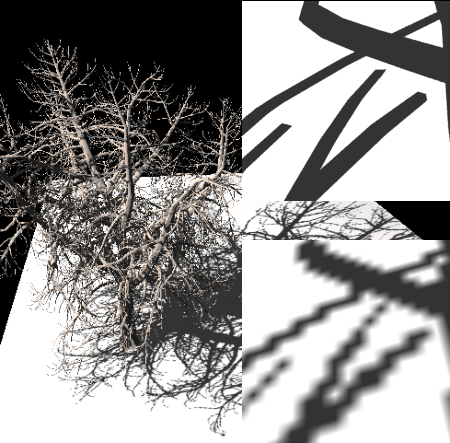
\includegraphics[height=5cm]{img/asm} \\
    Up right: ASM with a resolution of $131,072^2$. \\
    Down right: SM with a resolution of $2048^2$.
  \end{center}
\end{frame}

\begin{frame}
  \frametitle{Adaptive Shadow Map -- Performance}
  \begin{center}
    \begin{tabular}{c c c c c}
      PageSize & FPS & ASM L & ASM LMN & ASM LML \\\hline
      $8^2$ & 13.7 & 91\% & 77\% & 74\% \\
      $16^2$ & 15.6 & 90\% & 76\% & 73\% \\
      $32^2$ & 12.1 & 89\% & 75\% & 73\% \\
      $64^2$ & 12.9 & 89\% & 74\% & 73\% \\
    \end{tabular} \vspace{9mm}

    Performance relative to the SM with a resolution of $2048^2$.
  \end{center}
\end{frame}

\section{Results, conclusion, discussion}
\subsection{Results}
\begin{frame}
  \frametitle{Performance results}
  \begin{tabular}{l c c}
    Method & Cg ops & HW ops \\\hline
    \emph{Stream 1D→2D} &&\\
    ~~Glift, no specialization & 8 & 5 \\
    ~~Glift, with specialization & 5 & 4 \\
    ~~Hardcoded Cg & 4 & 3\\
    \emph{1D sparse, uniform 3D→3D page table} &&\\
    ~~Glift, no specialization & 11 & 8 \\
    ~~Glift, with specialization & 7 & 5 \\
    ~~Hardcoded Cg & 6 & 5\\
    \emph{Adaptive shadow map + offset} &&\\
    ~~Glift, no specialization & 31 & 10 \\
    ~~Glift, with specialization & 27 & 10 \\
    ~~Hardcoded Cg & 16 & 9\\
  \end{tabular}
\end{frame}

\begin{frame}
  \frametitle{Results}

  Little to no performance penalty. \pause However, driver optimization is highly
  used. May cause performance problems if your code is hard to optimize.
\end{frame}

\begin{frame}
  \frametitle{Discussion}

  \begin{itemize}
  \item<1-> Heavily uses templates and optimizers to create a usable data
    structure abstraction.
  \item<2-> Would be beneficial to have true pointers for the GPU iterators.
  \item<3-> Is limited to non-sequential data structures.
  \end{itemize}
\end{frame}

\begin{frame}
  \frametitle{Conclusion}

  \begin{itemize}
  \item<+-> Glift is a working implementation of an abstraction for data
    structures on the GPU.
  \item<+-> Enables GPU programmers to develop more complex GPU applications, as
    it's possible to manage the complexity using this abstraction.
  \item<+-> Seems likely that this will be more important in upcoming years.
  \item<+-> Doesn't give any huge performance penalties.
  \item<+-> Shows promising results, considering this is (was?) still a
    prototype.
  \end{itemize}
\end{frame}

\end{document}
